% Options for packages loaded elsewhere
\PassOptionsToPackage{unicode}{hyperref}
\PassOptionsToPackage{hyphens}{url}
\PassOptionsToPackage{dvipsnames,svgnames,x11names}{xcolor}
%
\documentclass[
  letterpaper,
  DIV=11,
  numbers=noendperiod]{scrartcl}

\usepackage{amsmath,amssymb}
\usepackage{lmodern}
\usepackage{iftex}
\ifPDFTeX
  \usepackage[T1]{fontenc}
  \usepackage[utf8]{inputenc}
  \usepackage{textcomp} % provide euro and other symbols
\else % if luatex or xetex
  \usepackage{unicode-math}
  \defaultfontfeatures{Scale=MatchLowercase}
  \defaultfontfeatures[\rmfamily]{Ligatures=TeX,Scale=1}
  \setmainfont[]{Garamond}
\fi
% Use upquote if available, for straight quotes in verbatim environments
\IfFileExists{upquote.sty}{\usepackage{upquote}}{}
\IfFileExists{microtype.sty}{% use microtype if available
  \usepackage[]{microtype}
  \UseMicrotypeSet[protrusion]{basicmath} % disable protrusion for tt fonts
}{}
\makeatletter
\@ifundefined{KOMAClassName}{% if non-KOMA class
  \IfFileExists{parskip.sty}{%
    \usepackage{parskip}
  }{% else
    \setlength{\parindent}{0pt}
    \setlength{\parskip}{6pt plus 2pt minus 1pt}}
}{% if KOMA class
  \KOMAoptions{parskip=half}}
\makeatother
\usepackage{xcolor}
\setlength{\emergencystretch}{3em} % prevent overfull lines
\setcounter{secnumdepth}{-\maxdimen} % remove section numbering
% Make \paragraph and \subparagraph free-standing
\ifx\paragraph\undefined\else
  \let\oldparagraph\paragraph
  \renewcommand{\paragraph}[1]{\oldparagraph{#1}\mbox{}}
\fi
\ifx\subparagraph\undefined\else
  \let\oldsubparagraph\subparagraph
  \renewcommand{\subparagraph}[1]{\oldsubparagraph{#1}\mbox{}}
\fi


\providecommand{\tightlist}{%
  \setlength{\itemsep}{0pt}\setlength{\parskip}{0pt}}\usepackage{longtable,booktabs,array}
\usepackage{calc} % for calculating minipage widths
% Correct order of tables after \paragraph or \subparagraph
\usepackage{etoolbox}
\makeatletter
\patchcmd\longtable{\par}{\if@noskipsec\mbox{}\fi\par}{}{}
\makeatother
% Allow footnotes in longtable head/foot
\IfFileExists{footnotehyper.sty}{\usepackage{footnotehyper}}{\usepackage{footnote}}
\makesavenoteenv{longtable}
\usepackage{graphicx}
\makeatletter
\def\maxwidth{\ifdim\Gin@nat@width>\linewidth\linewidth\else\Gin@nat@width\fi}
\def\maxheight{\ifdim\Gin@nat@height>\textheight\textheight\else\Gin@nat@height\fi}
\makeatother
% Scale images if necessary, so that they will not overflow the page
% margins by default, and it is still possible to overwrite the defaults
% using explicit options in \includegraphics[width, height, ...]{}
\setkeys{Gin}{width=\maxwidth,height=\maxheight,keepaspectratio}
% Set default figure placement to htbp
\makeatletter
\def\fps@figure{htbp}
\makeatother

\KOMAoption{captions}{tableheading}
\makeatletter
\@ifpackageloaded{tcolorbox}{}{\usepackage[many]{tcolorbox}}
\@ifpackageloaded{fontawesome5}{}{\usepackage{fontawesome5}}
\definecolor{quarto-callout-color}{HTML}{909090}
\definecolor{quarto-callout-note-color}{HTML}{0758E5}
\definecolor{quarto-callout-important-color}{HTML}{CC1914}
\definecolor{quarto-callout-warning-color}{HTML}{EB9113}
\definecolor{quarto-callout-tip-color}{HTML}{00A047}
\definecolor{quarto-callout-caution-color}{HTML}{FC5300}
\definecolor{quarto-callout-color-frame}{HTML}{acacac}
\definecolor{quarto-callout-note-color-frame}{HTML}{4582ec}
\definecolor{quarto-callout-important-color-frame}{HTML}{d9534f}
\definecolor{quarto-callout-warning-color-frame}{HTML}{f0ad4e}
\definecolor{quarto-callout-tip-color-frame}{HTML}{02b875}
\definecolor{quarto-callout-caution-color-frame}{HTML}{fd7e14}
\makeatother
\makeatletter
\makeatother
\makeatletter
\makeatother
\makeatletter
\@ifpackageloaded{caption}{}{\usepackage{caption}}
\AtBeginDocument{%
\ifdefined\contentsname
  \renewcommand*\contentsname{Table of contents}
\else
  \newcommand\contentsname{Table of contents}
\fi
\ifdefined\listfigurename
  \renewcommand*\listfigurename{List of Figures}
\else
  \newcommand\listfigurename{List of Figures}
\fi
\ifdefined\listtablename
  \renewcommand*\listtablename{List of Tables}
\else
  \newcommand\listtablename{List of Tables}
\fi
\ifdefined\figurename
  \renewcommand*\figurename{Figure}
\else
  \newcommand\figurename{Figure}
\fi
\ifdefined\tablename
  \renewcommand*\tablename{Table}
\else
  \newcommand\tablename{Table}
\fi
}
\@ifpackageloaded{float}{}{\usepackage{float}}
\floatstyle{ruled}
\@ifundefined{c@chapter}{\newfloat{codelisting}{h}{lop}}{\newfloat{codelisting}{h}{lop}[chapter]}
\floatname{codelisting}{Listing}
\newcommand*\listoflistings{\listof{codelisting}{List of Listings}}
\makeatother
\makeatletter
\@ifpackageloaded{caption}{}{\usepackage{caption}}
\@ifpackageloaded{subcaption}{}{\usepackage{subcaption}}
\makeatother
\makeatletter
\@ifpackageloaded{tcolorbox}{}{\usepackage[many]{tcolorbox}}
\makeatother
\makeatletter
\@ifundefined{shadecolor}{\definecolor{shadecolor}{rgb}{.97, .97, .97}}
\makeatother
\makeatletter
\makeatother
\ifLuaTeX
  \usepackage{selnolig}  % disable illegal ligatures
\fi
\IfFileExists{bookmark.sty}{\usepackage{bookmark}}{\usepackage{hyperref}}
\IfFileExists{xurl.sty}{\usepackage{xurl}}{} % add URL line breaks if available
\urlstyle{same} % disable monospaced font for URLs
\hypersetup{
  pdftitle={Riri in the Wild Zone},
  pdfauthor={Laura Isabel Sastoque Pabón},
  colorlinks=true,
  linkcolor={blue},
  filecolor={Maroon},
  citecolor={Blue},
  urlcolor={Blue},
  pdfcreator={LaTeX via pandoc}}

\title{Riri in the Wild Zone}
\usepackage{etoolbox}
\makeatletter
\providecommand{\subtitle}[1]{% add subtitle to \maketitle
  \apptocmd{\@title}{\par {\large #1 \par}}{}{}
}
\makeatother
\subtitle{A Distant Reading of Sapphic Urban Latin Music}
\author{Laura Isabel Sastoque Pabón}
\date{}

\begin{document}
\maketitle
\ifdefined\Shaded\renewenvironment{Shaded}{\begin{tcolorbox}[interior hidden, breakable, enhanced, boxrule=0pt, frame hidden, sharp corners, borderline west={3pt}{0pt}{shadecolor}]}{\end{tcolorbox}}\fi

\renewcommand*\contentsname{Table of contents}
{
\hypersetup{linkcolor=}
\setcounter{tocdepth}{3}
\tableofcontents
}
\begin{tcolorbox}[enhanced jigsaw, bottomrule=.15mm, coltitle=black, breakable, colframe=quarto-callout-important-color-frame, toptitle=1mm, leftrule=.75mm, opacityback=0, colbacktitle=quarto-callout-important-color!10!white, toprule=.15mm, bottomtitle=1mm, title=\textcolor{quarto-callout-important-color}{\faExclamation}\hspace{0.5em}{Important}, colback=white, rightrule=.15mm, left=2mm, titlerule=0mm, opacitybacktitle=0.6, arc=.35mm]
Follow this link for a full GitHub Repository of this project

Final Project Repository
\end{tcolorbox}

\hypertarget{introduction}{%
\subsection{\texorpdfstring{1
\textbf{Introduction}}{1 Introduction}}\label{introduction}}

In recent years, distant reading methods have earned popularity for the
analysis of literary texts. These methods hinge on the transformation of
text into features--- data that can be quantified, qualified, and
visualized using computational tools.\footnote{Maciej Eder, et
  al.~``Stylometry with R: A Package for Computational Text Analysis.''
  \emph{The R Journal 8} (January 1, 2016): 107--21.
  https://doi.org/10.32614/RJ-2016-007.} Often framed in methodological
opposition to close reading, distant reading has been scrutinized for
its impulse to automate interpretation, and as its name indicates, to
build distance between the reader and the text. However, scholars such
as Katherine Bode have theorized that distant reading does not stand in
opposition to close reading, but is rather a conceptual legacy of the
latter, which prioritizes the text as the ultimate source of
meaning.\footnote{Katherine Bode. ``The Equivalence of `Close' and
  `Distant' Reading; or, Toward a New Object for Data-Rich Literary
  History.'' \emph{Modern Language Quarterly} (Seattle) 78, no. 1
  (2017): 77--106. https://doi.org/10.1215/00267929-3699787.}
Furthermore, scholars have called attention to distant reading methods
for their ability to reduce the reader's bias when working with texts,
and for their potential to expand existing literary canons through a
wider, more transparent inquiry of literary material.\footnote{Natalie
  M. Houston. ``Distant Reading and Victorian Women's Poetry.'' In
  \emph{The Cambridge Companion to Victorian Women's Poetry,} 249--65.
  Cambridge University Press, 2019.
  https://doi.org/10.1017/9781316856543.017.} So far, the majority of
applications of distant reading in the digital humanities have had
literary texts as their objects of inquiry---novels, poems, even
television scripts.\footnote{Joanna Byszuk. ``The Voices of Doctor Who
  -- How Stylometry Can Be Useful in Revealing New Information About TV
  Series.'' \emph{Digital Humanities Quarterly} 014, no. 4 (December 20,
  2020).} However, what happens when the objects of a distant reading
study are not commonly considered ``literary''? What happens when these
texts are, in fact, not even meant to be read, but instead heard, and
danced to?

In fact, few studies have ventured into the realm of music wearing a
distant reading toolbelt. Those that do, contain little critical
reflection on the application of these methods to this new textual
manifestation.\footnote{See for instance Elizabeth Monzingo and Daniel
  Shanahan. ``The Expression of Self and Grief in the Nineteenth
  Century: An Analysis through Distant Readings.''
  \emph{Nineteenth-Century Music Review} 18, no. 1 (2021): 83--107.
  https://doi.org/10.1017/S1479409819000697.} This essay aims to embark
on the experimental task of conducting a distant reading of sapphic
urban Latin music with an open, yet critical lens. In recent years,
urban Latin music---known for its highly sexualized lyrics and
male-dominated industry---has been undergoing a
transformation.\footnote{Henceforth, urban Latin music is used as an
  umbrella term for reggaetón, trap Latino, dembow, bachata, merengue,
  among other styles used by the artists in the corpus.} Not only are
female artists earning more and more notoriety, but a subset of queer,
and particularly sapphic artists is also emerging.\footnote{In this
  essay, the use of the term ``sapphic'' is an intentional choice to
  encompass the variety of identities through which queer desire aimed
  at women presents itself in urban Latin music. This term is preferred
  as opposed to ``lesbian,'' since it includes artists who do not
  exclusively sing about women but have a few select songs that were
  included in the corpus. These artists include Cazzu, Maria Becerra,
  Karol G, among others. It is also preferred to the word ``queer,''
  since this essay does not encompass male artists who write about other
  men, who are also an emerging subset in the genre, albeit less
  recognized by the mainstream. The word ``sapphic'' is also meant to
  include transgender women who at times sing about other women, such as
  Villano Antillano.} In a genre where the hyper-sexualization of women
is a convention, it is pertinent to interrogate whether women singers
are appropriating or modifying the language. Do sapphic songs---
particularly, at a lyrical level--- frame desire in a similar way to
straight male artists, or are they creating a new lexical tradition that
breaks pre-existing conventions?

By conducting distant reading analyses such as text mining, this study
aims to understand the appropriations and transformations of language
that sapphic singers are utilizing to advance their specific agenda
within the genre. This study conducts this analysis, however, with the
knowledge that the methods of distant reading were not built to deal
with these types of texts.\footnote{Distant reading practices are, first
  of all, most advanced for the English language. Secondly, they are
  based on dictionaries compiled, in their majority, from newspaper
  sources, which contain fairly standard manifestations of language. See
  Hans Ole Hatzel, et al.~``Machine Learning in Computational Literary
  Studies.'' \emph{It - Information Technology} 65, no. 4--5 (August 1,
  2023): 200--217. \url{https://doi.org/10.1515/itit-2023-0041},
  pp.~201-202.} Urban Latin music song lyrics are slang-heavy, filled
with non-standard manipulations of the Spanish language. They are
repetitive, highly onomatopoeic, and at times play with the boundaries
between Spanish, English, and Portuguese.\footnote{Patricio Josué
  Velarde Dediós. ``Reguetón de mujeres para mujeres: dos caminos de
  empoderamiento.'' \emph{Antec: Revista Peruana de Investigación
  Musical} 5, no. 1 (August 14, 2021): 91--109.
  https://doi.org/10.62230/antec.v5i1.112.} Therefore, this essay will
not take distant reading as a direct path to knowledge-making but will
instead engage in a two-way negotiation with its affordances,
shortcomings, and future possibilities. In doing so, it argues that
sapphic artists are able to simultaneously imitate and eschew the
male-dominated language of desire in urban Latin music. In Elaine
Showalter's terms, the particular position of sapphic urban Latin music
as an emerging, yet highly genealogical subgroup, allows it to stand in
a superposition of the ``muted zone'' and the ``wild zone'' of women's
writing, distinguished by their relationality to male convention.

\hypertarget{sapphic-desire-in-urban-latin-music}{%
\subsection{\texorpdfstring{2 \textbf{Sapphic Desire in Urban Latin
Music}}{2 Sapphic Desire in Urban Latin Music}}\label{sapphic-desire-in-urban-latin-music}}

In the last decade, women artists have slowly been carving out a space
for themselves in urban Latin music. Previous literature has meditated
on the role of some of the pioneering women \emph{reggaetoneras}, such
as Ivy Queen.\footnote{Dara E. Goldman. ``Walk like a Woman, Talk like a
  Man: Ivy Queen's Troubling of Gender.'' \emph{Latino Studies} 15, no.
  4 (November 1, 2017): 439--57.
  https://doi.org/10.1057/s41276-017-0088-5.} In a genre that blatantly
advances men's utilization of women as mediums for interrelationality,
and as sexual, often less-than-human objects, women artists have had to
carefully tip-toe the conventions of the genre to cultivate their
careers. In their earliest interventions, women were relegated to
uncredited lyrical accompaniments or ad-libs in male-dominated songs. In
some of their early musical projects, women artists would often
accommodate to convention and portray themselves as the objects of male
desire.\footnote{Velarde Dediós, p.~92.} This was perhaps with the
exception of Ivy Queen, whose songs were marked by a reclamation of her
own sexual agency. A ``queer'' gender presentation, accompanied with a
low-pitched voice, also characterized her strategy.\footnote{Goldman,
  p.~448.} As Patricio Josué Velarde Dediós points out, this trend has
shifted since the mid-2010s, with artists such as Becky G, Natti
Natasha, and Karol G. This new wave is characterized by high levels of
collaboration amongst women artists, whereas before they would largely
collaborate with men. Furthermore, musical projects directly challenge
some of the dualities and encasings that women face in reggaetón. Such
is the case of Becky G's \emph{Mala Santa} album, which aims to
challenge the virgin/whore dichotomy.

Most recently, a further development in this trend of women's
participation has begun---the inclusion of sapphic artists. This has not
only signified the popularization of new, lesbian-identifying artists
such as Young Miko, but also the release of sapphic songs by artists who
mostly sing about heterosexual desire, such as with Karol G and Kali
Uchis' ``Labios Mordidos.'' This development poses new theoretical
challenges. How can women establish themselves as both subjects and
objects of desire in a sphere that was built through the homosocial
relations of men? To an extent, the answer to this question is
experimentation. Reggaetón bears very particular linguistic
characteristics---from the hegemonic character of Puerto Rican slang to
an established set of zoomorphic words to refer to women.\footnote{Pavlina
  Vankova. ``Studying the Vocabulary of Reggaeton Song Lyrics.''
  \emph{Topics in Linguistics} 23, no. 2 (2022): 63--88.
  \url{https://doi.org/10.2478/topling-2022-0012}; Angel
  Torres-Toukoumidis, et al.~``Computational Analysis of Latin Music
  Songs Through Tokenization. Case of Female Artists and Reggaeton.'' In
  \emph{Communication and Applied Technologies}, edited by Paulo Carlos
  López-López, et al, 527--35. Smart Innovation, Systems and
  Technologies. Singapore: Springer Nature, 2023.
  https://doi.org/10.1007/978-981-19-6347-6\_47.} Part of the way
sapphic artists are inserting themselves in this genre is by bending
these conventions or imagining new possibilities for the lexical space
of reggaetón.

It is this very space of inventiveness that theorists of sapphic desire
have previously encountered. In ``Refiguring Lesbian Desire,'' Elizabeth
Grosz engages in an experimental reflection of how we can reframe
lesbian desire away from male-centric, often phallocentric conceptions
of ``lack'' and ``absence''---of a gaping void waiting to be filled.
Grosz associates this way of thinking with Freud's psychoanalytic
theories, which conceive of desire in negative terms. Instead, Grosz
proposes a theory of desire borrowing from rhizomatic thinking, where it
is defined in terms of ``parts and bits and interconnections, {[}what{]}
is new, {[}what{]} is exploratory, that opens up further spaces, induces
further intensities, speeds up, enervates, and proliferates production
(production of the body, production of the world).''\footnote{Elizabeth
  Grosz. ``Refiguring Lesbian Desire.'' In Space, Time and Perversion.
  Routledge, 1995, p.~81.} In these terms, desire becomes a productive
force, a force that does not incur hierarchy but rather flattens it. A
force that inevitably engenders knowledge.\footnote{Grosz hints at this
  conclusion in the ominous ending to her essay, ``that is the most we
  can hope for from knowledge. Or desire'' (p.~81).}

This productive space of sapphic desire is perhaps what Elaine Showalter
was imagining when she theorized the ``wild zone'' of women's culture.
This is the space in women's experience, in their way of understanding
and engaging with the world, that is ``no man's land.'' Because all
spheres of society are mediated by male conventions, including language,
the wild zone might even be a space of foreign tongues, a space outside
the ``prison-house'' of language.\footnote{Elaine Showalter. ``Feminist
  Criticism in the Wilderness.'' \emph{Critical Inquiry} 8, no. 2
  (1981): 179--205, p.~194.} There is no corresponding wild zone for
men, since their conventions and structures already inform language as
we know it, and thus bear no mystery.\footnote{It must acknowledged that
  this theory represents gender in strictly binary terms, which does not
  align with the gender identifications of many of the artists included
  in the corpus. However, this theory is useful in its theorizing of a
  space of language---and naturally, desire---where men are not allowed
  access.} According to Showalter, the wild zone is just a metaphorical
proposition, because in reality most of women's writing---their
production---is mediated through the ``muted zone.'' In the muted zone,
``muted groups must mediate their beliefs through the allowable forms of
dominant structures.''\footnote{Showalter, p.~201.} Hence, Showalter
proposes that we think of women's writing as a double-voiced discourse,
that toggles the line between the muted and wild zones, and that goes
beyond the dualistic view that women writers either imitate their
predecessors or revise them.\footnote{Showalter, p.~204.}

When writing in the sphere of urban Latin music, women artists are
confronted with existing scripts of desire. In the ``prison-house'' of
urban Latin lyrics, to express desire for a woman almost inevitably
signifies her sexualization and reduction to non-human elements. This
conundrum is palpable in many of the recent hits of sapphic artists. In
an interview for \emph{Rolling Stone}, Young Miko discussed her debut EP
\emph{Trap Kitty} (2022). The songs follow Riri, a pole dancer working
at a strip club in Puerto Rico. Upon first sight, one may associate the
way Young Miko sings about Riri with the way most men in the genre sing
about women. In the song ``Riri,'' Young Miko sings:

\begin{longtable}[]{@{}
  >{\raggedright\arraybackslash}p{(\columnwidth - 2\tabcolsep) * \real{0.4194}}
  >{\raggedright\arraybackslash}p{(\columnwidth - 2\tabcolsep) * \real{0.5806}}@{}}
\toprule()
\endhead
\begin{minipage}[t]{\linewidth}\raggedright
\emph{Le toco su cuerpo, eso es lo que ella ama,}\\
\emph{y prende la webcam cuando está en su cama.}\\
\emph{(\ldots)}\\
\emph{Ella se va viral en IG cuando publica}\\
\emph{Me dijo que sus captions siempre me los dedica}\\
\emph{(\ldots)}\\
\emph{Pa' ver su contenido tienes que pagar el prime.}\strut
\end{minipage} & \begin{minipage}[t]{\linewidth}\raggedright
I touch her body, that's what she loves,\\
and she turns on her webcam when she's in bed\\
(\ldots)\\
She goes viral on Instagram when she posts,\\
she told me her captions are all for me.\\
(\ldots)\\
To watch her content, you must pay for a prime
{[}subscription{]}.\footnote{Translated by the author.}\strut
\end{minipage} \\
\bottomrule()
\end{longtable}

To a listener familiar with popular urban Latin songs, these lyrics are
reminiscent of a common trend in male-dominated songs---the overt
discussion of sexual work almost as a desirable trait in women. ~One
such song is ``Only Fans'' by Young Martino, Myke Towers, and
Lunay.\footnote{I would invite readers to watch the music video for this
  song, to get an even more apparent insight on the images of women
  advanced by these lyrics.}

\begin{longtable}[]{@{}
  >{\raggedright\arraybackslash}p{(\columnwidth - 2\tabcolsep) * \real{0.4756}}
  >{\raggedright\arraybackslash}p{(\columnwidth - 2\tabcolsep) * \real{0.5244}}@{}}
\toprule()
\endhead
\begin{minipage}[t]{\linewidth}\raggedright
\emph{Con el tiempo vi un vídeo por ahí}\\
\emph{Y en OnlyFans rápido me suscribí}\\
\emph{(\ldots)}\\
\emph{Y e' una santa en Instagram (así)}\\
\emph{Y e' una puta en OnlyFans (¡ah!)}\strut
\end{minipage} & \begin{minipage}[t]{\linewidth}\raggedright
In time, I saw a video laying around,\\
and quickly subscribed to her OnlyFans.\\
(\ldots)\\
She's a saint on Instagram,\\
but a whore on OnlyFans.\footnote{Translated by the author.}\strut
\end{minipage} \\
\bottomrule()
\end{longtable}

A non-attentive reader would be quick to group ``Riri'' among the set of
women's songs that primarily imitate men's language of desire. However,
Young Miko asserts that her music--- although ``raunchy''--- is meant
for women and queer folks.\footnote{Solá Santiago Frances ``Welcome to
  Young Miko's World.'' \emph{Rolling Stone} (blog), June 26, 2023.
  \url{https://www.rollingstone.com/music/music-features/young-miko-trap-kitty-bad-bunny-karol-g-1234771397/}.}
And upon closer inspection, it is possible to glean some of this
intentionality. Whereas ``Only Fans'' is largely about the male singer
``I,'' ``Riri'' predominantly endows its female character with agency,
speaking of what she loves, and only once using a reference to the ``I''
(even then, the pronoun is in its reflexive form `me' + verb). How many
more of these subtle differences, these delicate negotiations between
the muted and wild zones would we encounter if we were able to look at a
sapphic urban Latin music as a whole? Or, in realistic terms, if we
looked at a representative sample of the emerging phenomenon of sapphic
music, and examined it against a set of conventional, male-dominated
songs? This is where the methodologies of distant reading prove useful
for the question at hand. By building, quantifying, and visualizing a
corpus of song lyrics, we will engage with sapphic music's \emph{prise
de la parole,} which goes hand-in-hand with women writers' \emph{prise
de conscience.}\footnote{Showalter, p.~190.}

\hypertarget{the-creation-of-a-corpus-canon}{%
\subsection{\texorpdfstring{3 \textbf{The Creation of a
Corpus-Canon}}{3 The Creation of a Corpus-Canon}}\label{the-creation-of-a-corpus-canon}}

The selection of a representative corpus is a key step in any distant
reading analysis. This entity---the ``corpus''---stems from the field of
corpus linguistics, which aims ``to construct and empirically analyze a
sample of texts as the basis for the meaningful generalizations about a
language or discourse domain.''\footnote{Jesse Egbert, et
  al.~\emph{Designing and Evaluating Language Corpora: A Practical
  Framework for Corpus Representativeness}. Cambridge University Press,
  2022. \url{https://doi.org/10.1017/9781316584880}, pp.~5-6.} The
corpus describes not the ultimate goal of inquiry, but its method or
material. The corpus has a target---in this case, the domain of sapphic
urban Latin music. An imperfect analogue in close-reading-based literary
studies is perhaps the literary canon. Although a canon is constructed
through a historical process of scholarly inquiry, rather than
statistical sampling, it decidedly positions certain texts as
``representative'' of a movement or domain of literature. The literary
canon carries a certain air of authority that attracts scholars seeking
to understand a specific time period or moment in literary history. This
is similar to the process by which a corpus often gets reused by authors
seeking to reproduce or build on past scholars' contributions. Natalie
Houston builds on Annette Kolodny's ideas in stating that computational
feminist criticism allows for ``explicit reflection on the decisions
made in conducting the dataset.''\footnote{Houston, p.~251.} For
Houston, distant reading offers a departure away from literary canons
that are often examined uncritically. Showalter reaches a similar point,
in stating that feminist criticism at its core aimed to resist existing
canons.\footnote{Showalter, p.~182.} Therefore, scholars of
computational feminist criticism believe that a corpus, by making the
boundaries of selection explicit, bears advantages of representativity
over a literary canon.\footnote{Houston, p.~255.}

Nonetheless, the boundary between a corpus and a canon is one that
should be threaded carefully. As theorists of corpus linguistics have
suggested, it is perhaps just as easy to introduce bias into a corpus as
it is to drown in the incompleteness of a canon.\footnote{Egbert, et al.}
This realization was central in the process of creating a corpus for
this study. Delineating a corpus of sapphic songs in urban Latin music
was a challenging task. The artists are multifaceted---they differ in
terms of age, nationality, sexual identity, and artistic goals.
Likewise, the peculiarities of their lyrics sit in discomfort with the
requirements of a corpus analysis--- their texts are highly oral,
repetitive, and slang-heavy. In other words, even though sapphic urban
Latin music is bound together by a shared identity, it seems to resist
corpus-making, and by extension, canon-making. Part of the
self-reflective process of dataset creation was an active evaluation of
personal biases in artist-song selection, and an active effort to
counteract or balance these impulses. Appropriate selection criteria for
sapphic urban Latin songs are more complicated than looking at a chart
of the most popular artists and scraping their top songs. A selection
based on popularity would erase the work of smaller, emerging artists,
with rich and varying agendas and lexical possibilities. To select
artists based on popularity would be to conform to a canon advanced by
mainstream music industries, the same canon that women's writing has for
centuries attempted to resist. Therefore, the corpus-creation process
for this study was a constructive one. It began with the charts and thus
selected top songs by popular artists such as Young Miko, Karol G, and
María Becerra. Then, it took the time to scrutinize other areas where
emerging sapphic artists often promote their music. This included social
media and Spotify playlists and led to the inclusion of smaller artists
such as Chzter and Gudnana, as well as artists whose agenda is slightly
more activism-based, such as Chocolate Remix.

Admittedly, corpus creation also inevitably incurred decisions on the
exclusion of material. For instance, I took the decision to not include
sapphic artists from Spain, except when in collaboration with Latin
artists.\footnote{These include Rosalía and Tokischa's ``Linda,'' and
  Nicki Nicole, Snow Tha Product, and Ptazeta's ``Tengo To'.''} Although
several Spanish women singers are now ubiquitous in the Latin music
mainstream, the historical development of Spanish women's music is
markedly different from that of Latin America.\footnote{Simply put,
  there are a lot of female singers in Spain who sing sapphic lyrics
  than in Latin America, and their affiliations to the urban Latin
  sphere are blurry, making their inclusion an issue of
  representativity.} Therefore, their inclusion would introduce noise
and skew the corpus, which exceeds the scope of this study. Artists not
markedly within urban genres, but rather in indie variations, were also
not included in the scope of this study. The sampling strategy was also
affected by the fact that most lyrics were scraped from Genius, and
therefore limited by the songs available on the platform. However, an
effort was made to manually retrieve lyrics to lesser-known songs on
other online sites, such as AZlyrics. No songs were transcribed by ear,
although this remains a viable route in future studies. Lastly, a sample
of songs by men was also included in the corpus, to facilitate
comparative analysis. This sample was stratified to match the
nationalities of the women sub-corpus, since different Latin American
countries can bring drastically different vocabulary and slang to
song-writing.\footnote{Vankova.} Likewise, the sub-corpus includes
lesser-known male artists such as Dani Flow.

The resulting corpus contains 166 songs, of which 83 are predominantly
written by women, and 83 are written by men.\footnote{It is important to
  mention that not all singers in the corpus were the only songwriters
  of their songs. Some songs are written in collaboration with producers
  and other artists. However, the songs selected are ones that are
  evidently written predominantly by the (woman) performer.}~

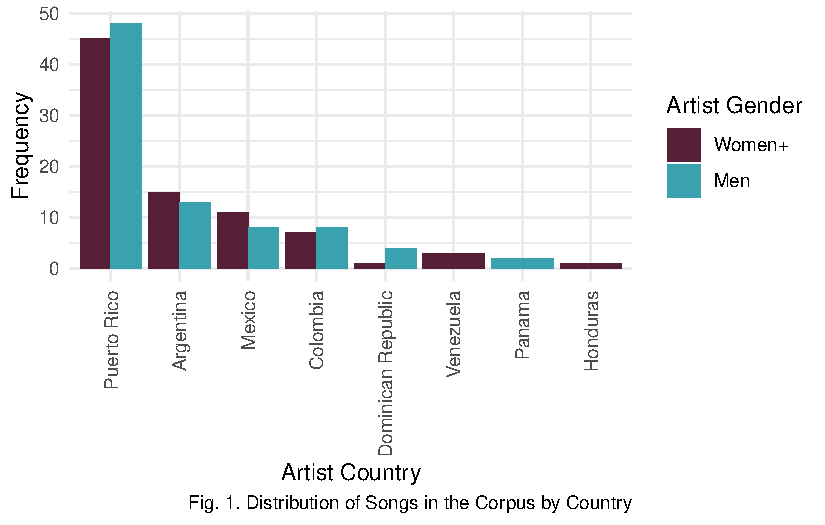
\includegraphics{Sastoque_Essay3_files/figure-pdf/songs-by-country-1.pdf}

However, this process still raised many questions. For instance, we may
be able to determine whether a song is written by a woman, but how can
we tell when a song is \emph{about} a woman, and consequently, sapphic?
Historically, sapphic singers have utilized different strategies to sing
about women without making it apparent. A good example is the case of
Ana Gabriel, who since the 1980s has been releasing songs about women,
but masked behind male pronouns, such as ``Simplemente Amigos'' (Just
Friends). ~Other songs forgo the gendered character of the Spanish
language by addressing their lyrics to a ``you,'' as is the case with
Karol G's ``CONTIGO.'' In this case, prudent decision-making was
implemented. For instance, ``CONTIGO'' is accompanied by a very
explicitly sapphic music video and was therefore included in the corpus.
Still, these complications of defining a ``sapphic'' song merit further
discussion, and I encourage future researchers to delve further into
this matter.

\hypertarget{results}{%
\subsection{\texorpdfstring{4
\textbf{Results}}{4 Results}}\label{results}}

The prospect of utilizing distant reading tools to understand the
``female shift'' in urban Latin music has interested previous
researchers. In 2022, Angel Torres-Toukoumidis and Isidro
Marin-Gutiérrez published a study titled ``Computational Analysis of
Latin Music Songs Through Tokenization: Case of Female Artists and
Reggaetón.'' This study compiled a corpus of 641 songs by 12
\emph{reggaetoneras} and conducted a lexical analysis of their
characteristics. Among their results, Torres-Toukoumidis and
Marin-Gutiérrez found that women's reggaetón presented a high index of
lexical diversity, where 4992 words were only used five
times.\footnote{Angel Torres-Toukoumidis, et al.~``Computational
  Analysis of Latin Music Songs Through Tokenization. Case of Female
  Artists and Reggaeton.'' In \emph{Communication and Applied
  Technologies}, edited by Paulo Carlos López-López, et al., 527--35.
  Smart Innovation, Systems and Technologies. Singapore: Springer
  Nature, 2023. \url{https://doi.org/10.1007/978-981-19-6347-6_47},
  p.~531.} The authors interpreted this finding as counter-evidence to
the popular belief that reggaetón is a genre with limited, simple
vocabulary. Furthermore, the authors also found a lower usage of
zoomorphic characteristics to self-designate, as is common in the
genre's discussion of women. Although this study offers an essential
introduction to the application of distant reading to urban Latin music,
there are many ways in which its methods could be taken a step further.

This study aims to fill some of these methodological gaps, and will also
offer a view into the narrower population of sapphic urban Latin songs.
In the first place, this study is based not only on a corpus of songs by
women, but also encompasses a comparative sub-corpus of songs by men
that will allow to draw direct comparisons between the two groups.
Secondly, this study will analyze a particular set of tokens that are
commonly used in urban Latin music to denote women and desire, and will
compare their usage and discourse across the two groups.

\hypertarget{frequencies}{%
\subsubsection{\texorpdfstring{4.1.
\textbf{Frequencies}}{4.1. Frequencies}}\label{frequencies}}

An appropriate first step when analyzing token frequency in our corpus,
is to visualize a simple word cloud of the most common words (Fig. 2).

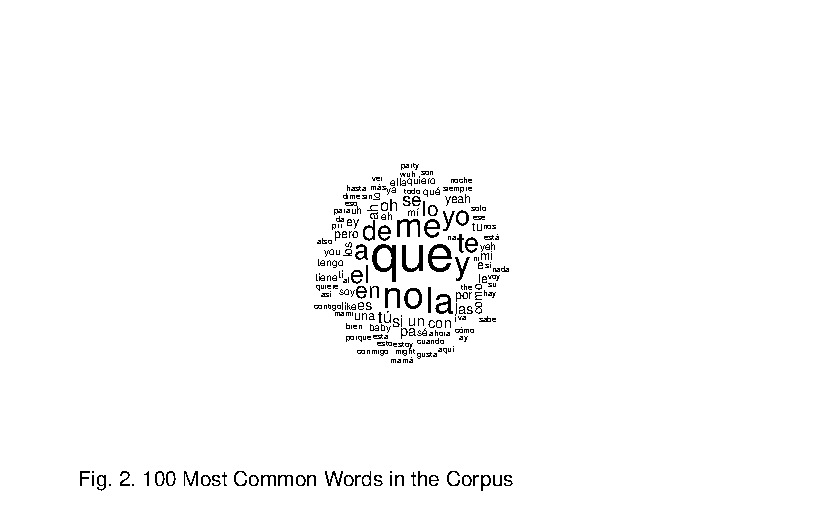
\includegraphics{Sastoque_Essay3_files/figure-pdf/word-cloud-1.pdf}

Similar to Fig. 47.1 in Torres-Toukoumidis, et al., the majority of the
most common words include common pronouns, articles, and conjunctions
found in the Spanish language. In order to make this visualization more
helpful to our research goals, we can delete stopwords. Since this
analysis uses \texttt{quanteda} tools in R, the stopwords deleted were
those found in the \texttt{stopwords} package. Due to the high usage of
English loanwords and expressions in urban Latin music, both Spanish and
English words were deleted. Then, the wordclouds were separated by
gender.

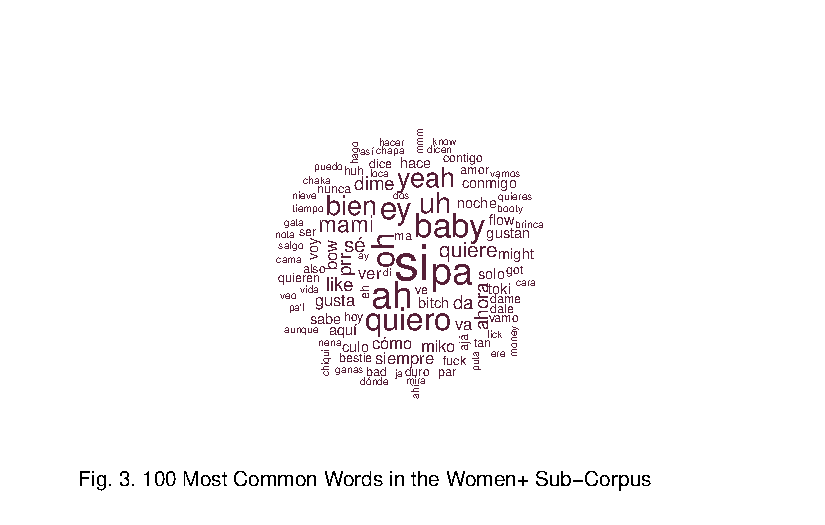
\includegraphics{Sastoque_Essay3_files/figure-pdf/word-cloud-by-gender-ns-1.pdf}

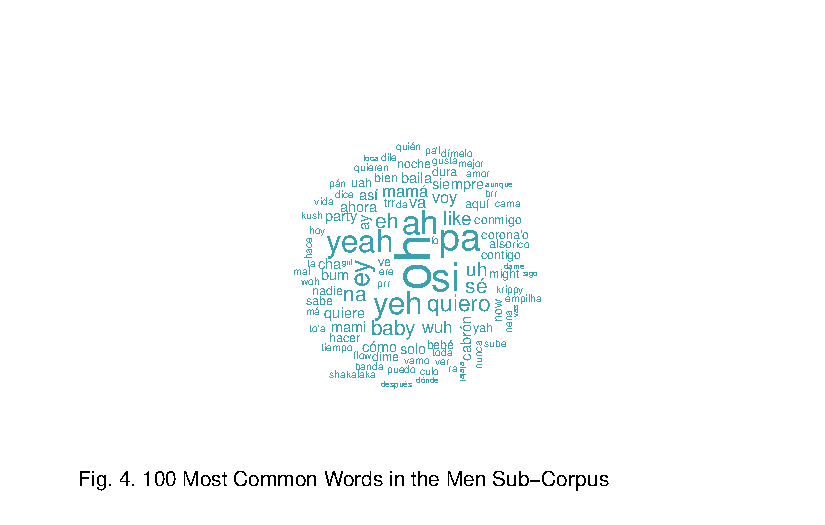
\includegraphics{Sastoque_Essay3_files/figure-pdf/word-cloud-by-gender-ns-2.pdf}

In \textbf{Fig. 3 and 4}, we can begin to glean some of the
particularities of working with urban Latin music specifically. This
includes a high number of onomatopeic vocabulary, such as ``oh,''
``wuh,'' and ``trr.'' Furthermore, for both groups we can see words
commonly used to refer to women, such as ``baby,'' and ``mami.'' In
both, but perhaps to a slightly more noticeable extent for women, words
with corporeal meaning appear, such as ``culo,'' ``dura,'' and ``chapa''
(ass, toned, ass).

Even though the cleaning of stopwords allows us to look into some of the
more specific vocabulary in the corpus, we can clearly see one of the
limitations of distant reading tools in working with urban music. Many
of the most frequent words in \textbf{Fig. 3} \textbf{and 4}, are in
fact contractions of stopwords that are commonly used in oral settings.
These include ``na,'' ``pa,'' and ``to'a'' which stand for ``nada,''
``para,'' and ``all (feminine).'' Since stopword lists currently
available for NLP (Natural Language Processing) are predominantly
compiled using written language, the tool was unable to detect these
contractions.

Furthermore, in much of urban music, it is common for artists to shout
out their own names or names of collaborators/producers within their
lyrics. In the cleaning process, I made a conscious decision not to take
out these so-called ``ad-libs,'' since according to previous literature,
a lot of women's voices in urban music have historically been relegated
to backing vocals.\footnote{Dediós, p.~92.} However, these instances are
visible in the above word clouds, as is the case with ``Miko'' (for
Young Miko) and ``Toki'' (for Tokischa).

To experiment with this limitation, I manually compiled a list of tokens
to remove from the analyses. These include common contractions of
stopwords in Spanish, and names of artists and producers. The list also
includes common onomatopeic tokens. A full list of removed words can be
found in the \texttt{useless\_words.txt} file in the Github Repository.

\textbf{Fig. 5.} below shows a comparison of the most used tokens for
both groups, before and after cleaning. In these plots, the y-axis was
converted from token frequency, to a measure of proportion. This is due
to the fact that, even though both sub-corpuses contain the same number
of songs, the men sub-corpus contained considerably more tokens. This
raises interesting questions regarding possible differences in song
length or singing speed between the two groups which merits further
scholarly inquiry. To avoid the artificial conclusions, proportions were
calculated by means of \(\frac{Token Frequency}{Total Subgroup Tokens}\)

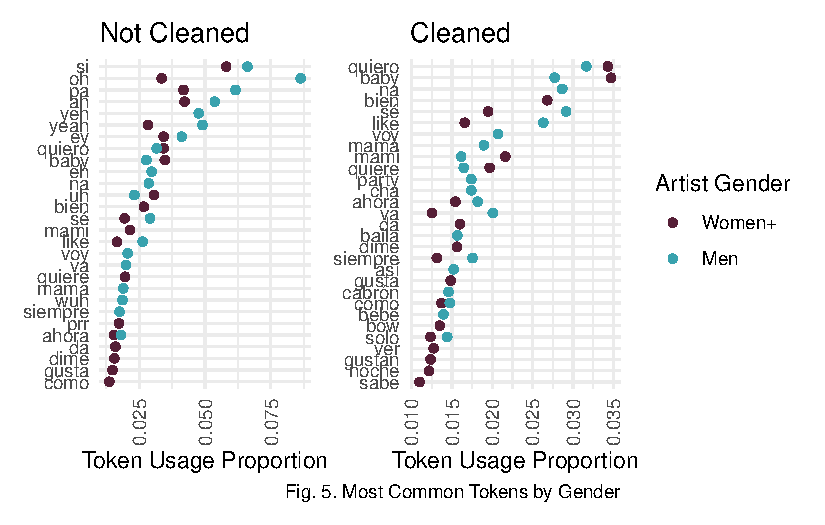
\includegraphics{Sastoque_Essay3_files/figure-pdf/prop-graph-1.pdf}

In the uncleaned facet, we can observe that some of the onomatopoeic
vocabulary seems to occupy a higher proportion of men's vocabulary in
the corpus, like in the face of ``oh'' and ``ah.'' However, other
onomatopoeic tokens, such as ``prr,'' are exclusively used by women.
So-called ``pet names'' for women such as ``baby'' and ``mami'' seem to
occupy a higher proportion of sapphic women's vocabulary. Words
exclusively used by men include ``party,'' ``baila'' (dance), and
``cabrón'' (Puerto Rican slang to denote `asshole', gendered male). This
could suggest that men are more keen to situate their songs within
party/club spaces. Words exclusively used by sapphic women include
``bien'' (good), ``dime'' (tell me), and ``gusta'' (he/she likes). These
direct addresses of the object of the song, and a reference to the
object's desires, could suggest that songs by women present a higher
engagement with the thoughts of the women to which their songs are
addressed. For instance, by quite literally asking them to speak.

Whether it is possible to compile a list of words to remove in a way
that is objective and does not introduce bias into the dataset is worthy
of reflection. The following analyses will work with the entire corpus,
including stopwords, since some of the words of interest include female
pronouns and articles, such as ``ella'' (she/her). For a full list of
words investigated, see \texttt{words\_of\_interest.txt} .

\textbf{Table 1} below shows a number of these results were interesting
comparisons were found across both groups. For instance, only the
sapphic women subcorpus uses the word ``bestie.'' Perhaps this could be
attributed to common storylines of friendship that exist in sapphic
songs. In contradiction, it was found that the men subcorpus uses the
word ``amiga'' (female friend) at a higher proportion. This
contradiction, and the meaning of these words in their specific context
will be investigated further. Relatively similar proportions were found
for tokens such as ``ella'' (her) and ``la'' (female article). Major
differences were found for the words ``bitch'' and ``booty.'' Along with
``bestie,'' this could suggest a general trend for the usage of words in
English to refer to women, especially with regards to the body. As noted
in \textbf{Fig. 5}, the word ``gusta'' (he/she likes) remains a notable
difference between the two groups.

\begin{longtable}[]{@{}lllllll@{}}
\caption{Table 1. Words of Interest Across both Groups}\tabularnewline
\toprule()
& Token & Frequency & Rank & Song\_Freq & Artist\_Gender & Proportion \\
\midrule()
\endfirsthead
\toprule()
& Token & Frequency & Rank & Song\_Freq & Artist\_Gender & Proportion \\
\midrule()
\endhead
5420 & amiga & 29 & 225 & 10 & Men & 0.0045 \\
344 & amiga & 13 & 331 & 10 & Women & 0.0025 \\
5231 & baby & 177 & 45 & 56 & Men & 0.0277 \\
27 & baby & 180 & 27 & 49 & Women & 0.0347 \\
114 & bestie & 43 & 112 & 3 & Women & 0.0083 \\
5857 & bitch & 9 & 646 & 6 & Men & 0.0014 \\
85 & bitch & 57 & 84 & 16 & Women & 0.0110 \\
6541 & booty & 4 & 1285 & 3 & Men & 0.0006 \\
136 & booty & 35 & 132 & 11 & Women & 0.0067 \\
5279 & conmigo & 80 & 92 & 29 & Men & 0.0125 \\
89 & conmigo & 56 & 86 & 29 & Women & 0.0108 \\
5234 & ella & 160 & 48 & 38 & Men & 0.0251 \\
34 & ella & 162 & 34 & 42 & Women & 0.0312 \\
5321 & gusta & 53 & 134 & 20 & Men & 0.0083 \\
64 & gusta & 77 & 64 & 29 & Women & 0.0148 \\
5189 & la & 1252 & 3 & 83 & Men & 0.1962 \\
4 & la & 845 & 4 & 81 & Women & 0.1629 \\
\bottomrule()
\end{longtable}

It is important to note, however, that at times these differences can be
attributed to specific authors. For instance, the token ``bitch'' and
its overrepresentation in the women's subcorpus can likely be attributed
to the artist Young Miko, as evidenced by \textbf{Fig. 6}. below.

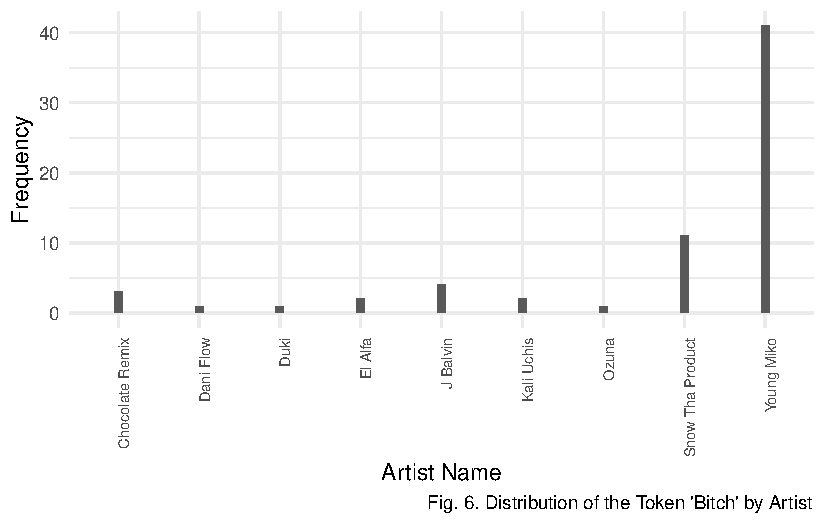
\includegraphics{Sastoque_Essay3_files/figure-pdf/by-author-1.pdf}

\hypertarget{concordances}{%
\subsubsection{4.2. Concordances}\label{concordances}}

Another tool in distant reading that can provide further insight into
our findings are concordances, which allow us to see the context in
which a certain token appears in the corpus.

In \textbf{Table 2 and 3} below, I decided to look into one of the most
sexualized terms to describe women in urban Latin music-- ``culo''
(ass). As evidenced by \textbf{Fig. 3 and 4}, this token was also among
the most common in both sub-corpuses. In these contexts, we can see a
certain level of lexical imitation from sapphic women. In many of these
cases, the word ``culo'' is used in conjunction with reflexive pronouns
such as ``me,'' which emphasize the effect of an action on the speaker.
In other words, both sub-corpuses seem to refer to women's bodies in
relation to the speaker's wants and desires. Furthermore, in the song
``Deseándote'' by Nath, the token is placed in cross proximity to
``Mercedes,'' engaging in a discourse of comparison of women with
objects.

\begin{longtable}[]{@{}
  >{\raggedright\arraybackslash}p{(\columnwidth - 8\tabcolsep) * \real{0.2991}}
  >{\raggedright\arraybackslash}p{(\columnwidth - 8\tabcolsep) * \real{0.2710}}
  >{\raggedright\arraybackslash}p{(\columnwidth - 8\tabcolsep) * \real{0.0748}}
  >{\raggedright\arraybackslash}p{(\columnwidth - 8\tabcolsep) * \real{0.2804}}
  >{\raggedright\arraybackslash}p{(\columnwidth - 8\tabcolsep) * \real{0.0748}}@{}}
\caption{Table 2. Concordance of the Token `Culo' in Men
Sub-Corpus}\tabularnewline
\toprule()
\begin{minipage}[b]{\linewidth}\raggedright
docname
\end{minipage} & \begin{minipage}[b]{\linewidth}\raggedright
pre
\end{minipage} & \begin{minipage}[b]{\linewidth}\raggedright
keyword
\end{minipage} & \begin{minipage}[b]{\linewidth}\raggedright
post
\end{minipage} & \begin{minipage}[b]{\linewidth}\raggedright
pattern
\end{minipage} \\
\midrule()
\endfirsthead
\toprule()
\begin{minipage}[b]{\linewidth}\raggedright
docname
\end{minipage} & \begin{minipage}[b]{\linewidth}\raggedright
pre
\end{minipage} & \begin{minipage}[b]{\linewidth}\raggedright
keyword
\end{minipage} & \begin{minipage}[b]{\linewidth}\raggedright
post
\end{minipage} & \begin{minipage}[b]{\linewidth}\raggedright
pattern
\end{minipage} \\
\midrule()
\endhead
La Jeepeta (Remix)\_Anuel AA & combi completa Ah Qué Chocha & culo &
teta Uah You might also & culo* \\
Tirando Flow Sesh \#11\_Dani Flow & Tie Tie Tie Tiene el & culo & grande
y la teta chica & culo* \\
Mírame (Remix)\_Rauw Alejandro & Que tú me mueves el & culo & rico en
eso estás vaqueá & culo* \\
Easy\_Jhayco & lo Baby y mueve ese & culo & berraco Así pégate Pégate
Así & culo* \\
Todo De Ti\_Rauw Alejandro & to eso completo De ese & culo & me volví un
teco eh & culo* \\
\bottomrule()
\end{longtable}

\begin{longtable}[]{@{}
  >{\raggedright\arraybackslash}p{(\columnwidth - 8\tabcolsep) * \real{0.3426}}
  >{\raggedright\arraybackslash}p{(\columnwidth - 8\tabcolsep) * \real{0.2778}}
  >{\raggedright\arraybackslash}p{(\columnwidth - 8\tabcolsep) * \real{0.0741}}
  >{\raggedright\arraybackslash}p{(\columnwidth - 8\tabcolsep) * \real{0.2315}}
  >{\raggedright\arraybackslash}p{(\columnwidth - 8\tabcolsep) * \real{0.0741}}@{}}
\caption{Table 3. Concordance of the Token `Culo' in Women
Sub-Corpus}\tabularnewline
\toprule()
\begin{minipage}[b]{\linewidth}\raggedright
docname
\end{minipage} & \begin{minipage}[b]{\linewidth}\raggedright
pre
\end{minipage} & \begin{minipage}[b]{\linewidth}\raggedright
keyword
\end{minipage} & \begin{minipage}[b]{\linewidth}\raggedright
post
\end{minipage} & \begin{minipage}[b]{\linewidth}\raggedright
pattern
\end{minipage} \\
\midrule()
\endfirsthead
\toprule()
\begin{minipage}[b]{\linewidth}\raggedright
docname
\end{minipage} & \begin{minipage}[b]{\linewidth}\raggedright
pre
\end{minipage} & \begin{minipage}[b]{\linewidth}\raggedright
keyword
\end{minipage} & \begin{minipage}[b]{\linewidth}\raggedright
post
\end{minipage} & \begin{minipage}[b]{\linewidth}\raggedright
pattern
\end{minipage} \\
\midrule()
\endhead
Besties (Remix)\_Young Miko & completa las modifico Qué Eso & culo & dan
un cien lo certifico & culo* \\
Brinca\_Young Miko & she's litty Uh Culo grande & culo & Iggy Rrr Que la
busque & culo* \\
Deseándote\_Nath & Pa qué Mercedes con ese & culote & Y cuando se suelta
más & culo* \\
ID\_Young Miko & Ja Perreando duro pégame ese & culo & Echa eso pa'cá
canto e & culo* \\
Labios Mordidos\_Kali Uchis \& KAROL G & Dios me le bendiga ese & culo &
que se pega uh uh & culo* \\
\bottomrule()
\end{longtable}

Concordances can also help us understand the role of the word ``amiga''
(female friend) in both groups. In the previous section, we observed how
the sapphic subcorpus exclusives uses the word ``bestie'', but includes
a lower proportion of the word ``amiga.'' \textbf{Table 4 and 5} reveal
a key distinction. In the men subcorpus, the word ``amiga'' is used to
refer to a woman's friends, towards whom the singer is hoping to make
sexual advances. In songs such as Bad Bunny's ``Titi Me Preguntó,'' the
figure of the female friend is mentioned as a potential ``guide'' who
could advise the woman not to get together with Bad Bunny, because of
his commitment issues. By contrast, in several instances of the sapphic
subcorpus, the word is used to describe an unsatisfactory friendship
that the singer desires to be romantic. Such is the case in Gudnana's
AMG ``que ladilla aparentar que solo somos amigas'' (how upsetting to
pretend that we are just friends).

\begin{longtable}[]{@{}
  >{\raggedright\arraybackslash}p{(\columnwidth - 8\tabcolsep) * \real{0.3679}}
  >{\raggedright\arraybackslash}p{(\columnwidth - 8\tabcolsep) * \real{0.2264}}
  >{\raggedright\arraybackslash}p{(\columnwidth - 8\tabcolsep) * \real{0.0755}}
  >{\raggedright\arraybackslash}p{(\columnwidth - 8\tabcolsep) * \real{0.2547}}
  >{\raggedright\arraybackslash}p{(\columnwidth - 8\tabcolsep) * \real{0.0755}}@{}}
\caption{Table 4. Concordance of the Token `Amiga' in Men
Sub-Corpus}\tabularnewline
\toprule()
\begin{minipage}[b]{\linewidth}\raggedright
docname
\end{minipage} & \begin{minipage}[b]{\linewidth}\raggedright
pre
\end{minipage} & \begin{minipage}[b]{\linewidth}\raggedright
keyword
\end{minipage} & \begin{minipage}[b]{\linewidth}\raggedright
post
\end{minipage} & \begin{minipage}[b]{\linewidth}\raggedright
pattern
\end{minipage} \\
\midrule()
\endfirsthead
\toprule()
\begin{minipage}[b]{\linewidth}\raggedright
docname
\end{minipage} & \begin{minipage}[b]{\linewidth}\raggedright
pre
\end{minipage} & \begin{minipage}[b]{\linewidth}\raggedright
keyword
\end{minipage} & \begin{minipage}[b]{\linewidth}\raggedright
post
\end{minipage} & \begin{minipage}[b]{\linewidth}\raggedright
pattern
\end{minipage} \\
\midrule()
\endhead
Con Calma\_Daddy Yankee & pa mí Dile a tus & amigas & que andamo ready
Sube Esto & amiga* \\
Baila Baila Baila (Remix)\_Daddy Yankee & va en busca de sus & amigas &
que la noche es pasajera & amiga* \\
Easy\_Jhayco & No le diga a tu & amiga & que estoy dándote que Se &
amiga* \\
Soltera (Remix)\_Daddy Yankee & Tá soltera Fuego con su & amiga &
revuelta Va pa la disco & amiga* \\
No Fue (Remix)\_Rauw Alejandro & Y girl dile a tu & amiga & que me haga
coro Que & amiga* \\
\bottomrule()
\end{longtable}

\begin{longtable}[]{@{}
  >{\raggedright\arraybackslash}p{(\columnwidth - 8\tabcolsep) * \real{0.2788}}
  >{\raggedright\arraybackslash}p{(\columnwidth - 8\tabcolsep) * \real{0.3077}}
  >{\raggedright\arraybackslash}p{(\columnwidth - 8\tabcolsep) * \real{0.0769}}
  >{\raggedright\arraybackslash}p{(\columnwidth - 8\tabcolsep) * \real{0.2596}}
  >{\raggedright\arraybackslash}p{(\columnwidth - 8\tabcolsep) * \real{0.0769}}@{}}
\caption{Table 5. Concordance of the Token `Amiga' in Women
Sub-Corpus}\tabularnewline
\toprule()
\begin{minipage}[b]{\linewidth}\raggedright
docname
\end{minipage} & \begin{minipage}[b]{\linewidth}\raggedright
pre
\end{minipage} & \begin{minipage}[b]{\linewidth}\raggedright
keyword
\end{minipage} & \begin{minipage}[b]{\linewidth}\raggedright
post
\end{minipage} & \begin{minipage}[b]{\linewidth}\raggedright
pattern
\end{minipage} \\
\midrule()
\endfirsthead
\toprule()
\begin{minipage}[b]{\linewidth}\raggedright
docname
\end{minipage} & \begin{minipage}[b]{\linewidth}\raggedright
pre
\end{minipage} & \begin{minipage}[b]{\linewidth}\raggedright
keyword
\end{minipage} & \begin{minipage}[b]{\linewidth}\raggedright
post
\end{minipage} & \begin{minipage}[b]{\linewidth}\raggedright
pattern
\end{minipage} \\
\midrule()
\endhead
AMG\_Gudnana & ladilla aparentar que solo como & amiga & yo quero
tenerte Aunque al & amiga* \\
Dime Como Hago\_Maria Becerra & Y no quiero ser tu & amiga & Quiero ser
la persona que & amiga* \\
Dime Como Hago\_Maria Becerra & Y no quiero ser tu & amiga & Quiero ser
la persona que & amiga* \\
Linda\_Tokischa \& Rosalía & estaba con La ROSALÍA Las & amigas & que se
besan son la & amiga* \\
Linda\_Tokischa \& Rosalía & estaba con La ROSALÍA Las & amigas & que se
besan son la & amiga* \\
\bottomrule()
\end{longtable}

It is also possible to investigate the context of multi-word phrases
using concordances. In this case, I was interested in delving further
into the differences in the use of reflexivity. For instance, the
varying proportion of the token ``gusta'' (he/she likes) raises
questions on the focus on subject versus object in each of these cases.
For this experiment, I analyzed the phrases ``ella me'' and ``ella se.''
The former uses the first-person reflexive pronoun to indicate that the
``she'' is conducting an action aimed towards the speaker. The latter
uses the third-person reflexive pronoun to indicate that she is
conducting an action aimed at herself. The first observation we can make
is that, while the sapphic subcorpus presents a comparable number of
instances of both ``ella me'' and ``ella se,'' the men's subcorpus
presents a notably higher number of ``ella me'' instances. This could
perhaps gesture towards a tendency for more protagonism of the singer in
the discourse of the song for the case of the male subcorpus.

\begin{longtable}[]{@{}
  >{\raggedright\arraybackslash}p{(\columnwidth - 8\tabcolsep) * \real{0.3440}}
  >{\raggedright\arraybackslash}p{(\columnwidth - 8\tabcolsep) * \real{0.2800}}
  >{\raggedright\arraybackslash}p{(\columnwidth - 8\tabcolsep) * \real{0.0640}}
  >{\raggedright\arraybackslash}p{(\columnwidth - 8\tabcolsep) * \real{0.2480}}
  >{\raggedright\arraybackslash}p{(\columnwidth - 8\tabcolsep) * \real{0.0640}}@{}}
\caption{Table 5. Concordance of the Phrase `Ella Me' in Men
Sub-Corpus}\tabularnewline
\toprule()
\begin{minipage}[b]{\linewidth}\raggedright
docname
\end{minipage} & \begin{minipage}[b]{\linewidth}\raggedright
pre
\end{minipage} & \begin{minipage}[b]{\linewidth}\raggedright
keyword
\end{minipage} & \begin{minipage}[b]{\linewidth}\raggedright
post
\end{minipage} & \begin{minipage}[b]{\linewidth}\raggedright
pattern
\end{minipage} \\
\midrule()
\endfirsthead
\toprule()
\begin{minipage}[b]{\linewidth}\raggedright
docname
\end{minipage} & \begin{minipage}[b]{\linewidth}\raggedright
pre
\end{minipage} & \begin{minipage}[b]{\linewidth}\raggedright
keyword
\end{minipage} & \begin{minipage}[b]{\linewidth}\raggedright
post
\end{minipage} & \begin{minipage}[b]{\linewidth}\raggedright
pattern
\end{minipage} \\
\midrule()
\endhead
Chica Paranormal\_Paulo Londra & punto de consumirme Pero cuando & ella
me & llama Wouh Olvidamo todo ahí & ella me \\
Chica Paranormal\_Paulo Londra & nuestro momento Pe Pero cuando & ella
me & llama Brr Olvidamo todo ahí & ella me \\
Chica Paranormal\_Paulo Londra & má Wouh Cada ve que & ella me & mira
tiene algo que me & ella me \\
Chica Paranormal\_Paulo Londra & nuestro momento Pe Pero cuando & ella
me & llama Olvidamo todo ahí en & ella me \\
Chica Paranormal\_Paulo Londra & de consumirme Ay Pero cuando & ella me
& llama Olvidamo todo ahí en & ella me \\
Chica Paranormal\_Paulo Londra & momento Yeh Pe Pero cuando & ella me &
llama Me llama qué Olvidamo & ella me \\
China\_Daddy Yankee & estaba contigo perreando Y de & ella me & olvidé
Mami Dios mío perdóname & ella me \\
China\_Daddy Yankee & la disco perreando Y con & ella me & enredé Woh oh
oh fuego & ella me \\
China\_Daddy Yankee & Tú me dejaste caer pero & ella me & levantó Uah
Déjame poca mujer & ella me \\
China\_Daddy Yankee & Uah Déjame poca mujer pero & ella me & levantó Oh
oh oh Y & ella me \\
China\_Daddy Yankee & estaba contigo perreando Y de & ella me & olvidé
Mami Dios mío perdóname & ella me \\
China\_Daddy Yankee & la disco perreando Y con & ella me & enredé Woh oh
oh fuego & ella me \\
China\_Daddy Yankee & la disco perreando Cuando con & ella me & envolví
sí Wuh wuh Mi & ella me \\
China\_Daddy Yankee & estaba contigo perreando Y de & ella me & olvidé
Mami Dios mío perdóname & ella me \\
China\_Daddy Yankee & la disco perreando Y con & ella me & enredé Woh oh
oh fuego & ella me \\
La Mamá de la Mamá\_El Alfa & descendencia entera Por qué Porque & ella
me & da La mamá de la & ella me \\
La Mamá de la Mamá\_El Alfa & bai bain Con la boca & ella me & lleva pa
Dubái bái Chikiri & ella me \\
La Mamá de la Mamá\_El Alfa & bai bain Con la boca & ella me & lleva pa
Dubái bái Dale & ella me \\
Loca (Remix)\_Duki & Y yo la toco y & ella me & toca No quiere a otro &
ella me \\
Me Tiene Mal\_Paulo Londra & tiene jodido Sólo pienso en & ella me &
siento perdido Sí Me importa & ella me \\
Mírame (Remix)\_Rauw Alejandro & y yo voy voy voy & Ella me & pide que
la castigue Tá & ella me \\
Qué Más Pues (Remix)\_Sech & Pri yah yah yah Farru & Ella me & escribió
después que la guayé & ella me \\
Suave (Remix)\_El Alfa & báilame en el tubo suave & Ella me & dice que
le gustan lo & ella me \\
Suave (Remix)\_El Alfa & le gustan lo plátano Maduro & Ella me & dice
que le gustan lo & ella me \\
Suave (Remix)\_El Alfa & le gustan lo plátano Maduro & Ella me & dice
que le gustan lo & ella me \\
Te Boté (Remix)\_Bad Bunny & amiga me textea siempre que & ella me &
desea Se tira una foto & ella me \\
Tirando Flow Sesh \#11\_Dani Flow & escote Brr Me dice MOTOPAPI & ella
me & pide que la azote Soy & ella me \\
Tirando Flow Sesh \#11\_Dani Flow & escote Jaja Me dice MOTOPAPI & ella
me & pide que la azote Pa & ella me \\
TRAPPERZ A Mafia Da Sicilia\_Rauw Alejandro & quítate del medio Ye yeah
& Ella me & están chequeando como TSA TSA & ella me \\
\bottomrule()
\end{longtable}

\begin{longtable}[]{@{}
  >{\raggedright\arraybackslash}p{(\columnwidth - 8\tabcolsep) * \real{0.3333}}
  >{\raggedright\arraybackslash}p{(\columnwidth - 8\tabcolsep) * \real{0.3070}}
  >{\raggedright\arraybackslash}p{(\columnwidth - 8\tabcolsep) * \real{0.0702}}
  >{\raggedright\arraybackslash}p{(\columnwidth - 8\tabcolsep) * \real{0.2193}}
  >{\raggedright\arraybackslash}p{(\columnwidth - 8\tabcolsep) * \real{0.0702}}@{}}
\caption{Table 6. Concordance of the Token `Ella Me' in Women
Sub-Corpus}\tabularnewline
\toprule()
\begin{minipage}[b]{\linewidth}\raggedright
docname
\end{minipage} & \begin{minipage}[b]{\linewidth}\raggedright
pre
\end{minipage} & \begin{minipage}[b]{\linewidth}\raggedright
keyword
\end{minipage} & \begin{minipage}[b]{\linewidth}\raggedright
post
\end{minipage} & \begin{minipage}[b]{\linewidth}\raggedright
pattern
\end{minipage} \\
\midrule()
\endfirsthead
\toprule()
\begin{minipage}[b]{\linewidth}\raggedright
docname
\end{minipage} & \begin{minipage}[b]{\linewidth}\raggedright
pre
\end{minipage} & \begin{minipage}[b]{\linewidth}\raggedright
keyword
\end{minipage} & \begin{minipage}[b]{\linewidth}\raggedright
post
\end{minipage} & \begin{minipage}[b]{\linewidth}\raggedright
pattern
\end{minipage} \\
\midrule()
\endhead
8 AM\_Young Miko & mi sombra Sombra Que Que & ella me & busque a mí eso
no & ella me \\
Castigada\_Young Miko & la otra Y más cuando & ella me & toca Toca Por
eso yo & ella me \\
Castigada\_Young Miko & la otra Y más cuando & ella me & toca Por eso yo
me & ella me \\
Condado\_Young Miko & tú ere injusta Spicy mami & ella me & usa Y no me
quejo & ella me \\
De Pasajero\_Young Miko & habla francé entonce habla english & Ella me &
dice monsieur Yeah de su & ella me \\
ID\_Young Miko & maybe no se acuerda Pero & ella me & dijo que era fan
de & ella me \\
ID\_Young Miko & Yeah yeah yeah Miko Pero & ella me & dijo que era fan
de & ella me \\
ID\_Young Miko & maybe no se acuerda Pero & ella me & dijo que era fan
de & ella me \\
Kachipun\_Young Miko & me salieron a cinco Y & ella me & los quita si le
gusta & ella me \\
Linda\_Tokischa \& Rosalía & le canto por bachata y & ella me & canta
por bulería Tú ere & ella me \\
Muñekita\_Kali Uchis & llena e boto Pero cuando & ella me & lo mueve ahí
es que & ella me \\
Muñekita\_Kali Uchis & el que tu nalga comanda & Ella me & llama porque
yo soy su & ella me \\
Que Le Gusta el Flow\_Snow Tha Product & Punta Cana to'a la semana &
Ella me & lo para como una vara & ella me \\
\bottomrule()
\end{longtable}

\begin{longtable}[]{@{}
  >{\raggedright\arraybackslash}p{(\columnwidth - 8\tabcolsep) * \real{0.2735}}
  >{\raggedright\arraybackslash}p{(\columnwidth - 8\tabcolsep) * \real{0.2650}}
  >{\raggedright\arraybackslash}p{(\columnwidth - 8\tabcolsep) * \real{0.0684}}
  >{\raggedright\arraybackslash}p{(\columnwidth - 8\tabcolsep) * \real{0.3248}}
  >{\raggedright\arraybackslash}p{(\columnwidth - 8\tabcolsep) * \real{0.0684}}@{}}
\caption{Table 7. Concordance of the Token `Ella Se' in Men
Sub-Corpus}\tabularnewline
\toprule()
\begin{minipage}[b]{\linewidth}\raggedright
docname
\end{minipage} & \begin{minipage}[b]{\linewidth}\raggedright
pre
\end{minipage} & \begin{minipage}[b]{\linewidth}\raggedright
keyword
\end{minipage} & \begin{minipage}[b]{\linewidth}\raggedright
post
\end{minipage} & \begin{minipage}[b]{\linewidth}\raggedright
pattern
\end{minipage} \\
\midrule()
\endfirsthead
\toprule()
\begin{minipage}[b]{\linewidth}\raggedright
docname
\end{minipage} & \begin{minipage}[b]{\linewidth}\raggedright
pre
\end{minipage} & \begin{minipage}[b]{\linewidth}\raggedright
keyword
\end{minipage} & \begin{minipage}[b]{\linewidth}\raggedright
post
\end{minipage} & \begin{minipage}[b]{\linewidth}\raggedright
pattern
\end{minipage} \\
\midrule()
\endhead
Easy\_Jhayco & Toítas puesta pa'l mismo sateo & Ella se & pegó y me
decía Así & ella se \\
Easy\_Jhayco & Toítas puesta pa'l mismo sateo & Ella se & pegó y me
decía Así & ella se \\
Gasolina\_Daddy Yankee & algo y lo sabe Conmigo & ella se & pierde No le
rinde cuentas & ella se \\
Gasolina\_Daddy Yankee & algo y lo sabe Conmigo & ella se & pierde No le
rinde cuentas & ella se \\
Tirando Flow Sesh \#11\_Dani Flow & no se le reza a & ella se & le
deposita Ando tirando flow & ella se \\
Tirando Flow Sesh \#11\_Dani Flow & no se le reza a & ella se & le
deposita Destápate acércate bájate & ella se \\
\bottomrule()
\end{longtable}

\begin{longtable}[]{@{}
  >{\raggedright\arraybackslash}p{(\columnwidth - 8\tabcolsep) * \real{0.3304}}
  >{\raggedright\arraybackslash}p{(\columnwidth - 8\tabcolsep) * \real{0.2589}}
  >{\raggedright\arraybackslash}p{(\columnwidth - 8\tabcolsep) * \real{0.0714}}
  >{\raggedright\arraybackslash}p{(\columnwidth - 8\tabcolsep) * \real{0.2679}}
  >{\raggedright\arraybackslash}p{(\columnwidth - 8\tabcolsep) * \real{0.0714}}@{}}
\caption{Table 8. Concordance of the Token `Ella Se' in Women
Sub-Corpus}\tabularnewline
\toprule()
\begin{minipage}[b]{\linewidth}\raggedright
docname
\end{minipage} & \begin{minipage}[b]{\linewidth}\raggedright
pre
\end{minipage} & \begin{minipage}[b]{\linewidth}\raggedright
keyword
\end{minipage} & \begin{minipage}[b]{\linewidth}\raggedright
post
\end{minipage} & \begin{minipage}[b]{\linewidth}\raggedright
pattern
\end{minipage} \\
\midrule()
\endfirsthead
\toprule()
\begin{minipage}[b]{\linewidth}\raggedright
docname
\end{minipage} & \begin{minipage}[b]{\linewidth}\raggedright
pre
\end{minipage} & \begin{minipage}[b]{\linewidth}\raggedright
keyword
\end{minipage} & \begin{minipage}[b]{\linewidth}\raggedright
post
\end{minipage} & \begin{minipage}[b]{\linewidth}\raggedright
pattern
\end{minipage} \\
\midrule()
\endhead
8 AM\_Young Miko & eso no me asombra Asombra & Ella se & va a arrepentir
si me & ella se \\
Chapa\_Valen Etchegoyen & chapa You might also like & Ella se & viste de
clase Diferente a & ella se \\
DISPO\_Young Miko & a la bebé Puesta pa & ella se & le ve Que ella sabe
& ella se \\
DISPO\_Young Miko & dura la bebé Puesta pa & ella se & le ve Que ella
sabe & ella se \\
Hipnotiza\_Maria Becerra & que el de nuestra frecuencia & Ella se &
desnuda yo soy su audiencia & ella se \\
Labios Mordidos\_Kali Uchis \& KAROL G & Y solo con mi mirá & ella se &
puso mojá Tu novia se & ella se \\
Riri\_Young Miko & emoji yo sé que significa & Ella se & va viral en IG
cuando & ella se \\
Riri\_Young Miko & siempre me los dedica ah & Ella se & enrola varios
siempre está on & ella se \\
Riri\_Young Miko & emoji yo sé que significa & Ella se & va viral en IG
cuando & ella se \\
Wiggy\_Young Miko & let's go Aserejé ja dejé & Ella se & dejó y yo me la
& ella se \\
Wiggy\_Young Miko & let's go Aserejé ja dejé & Ella se & dejó y yo me la
& ella se \\
Wiggy\_Young Miko & let's go Aserejé ja dejé & Ella se & dejó y yo me la
& ella se \\
\bottomrule()
\end{longtable}

\hypertarget{keyness}{%
\subsubsection{\texorpdfstring{4.3
\textbf{Keyness}}{4.3 Keyness}}\label{keyness}}

One more test that we can run to look into the matter of lexical
comparisons is a keyness test. This tool conducts a Chi-Squared
statistical test to determine which words may distinguish a given group
from another.

In \textbf{Fig. 7}., after removing our list of selected words, we can
see some of the words we have already been investigating, such as
``gustan,'' ``bestie,'' and ``bitch.'' However, due to the nature of the
corpus, we can also see names that are quite distinctly associated with
specific songs, such as ``Chulo'' and ``Brinca.'' The use of English
words such as ``booty'' and ``lick'' is noteworthy.

A keyness test is most commonly used to understand distinctions for
specific authors relative to a corpus. For the purposes of
experimentation, I separated out the Mexican sapphic artist Chzter. In
\textbf{Fig. 8,} we can see that the key tokens for distinction are
often thematic to her specific songs. ``Marciana'' (Martian) is often
used in the song ``Mátame Marciana,'' and the word ``lick'' is endemic
to the song ``LICK MY PSSY.'' Therefore, it is valuable to question how
much of these words' distinctiveness can be attributed to individual
artists' choices in their personal projects, rather than their adherence
to a general movement.

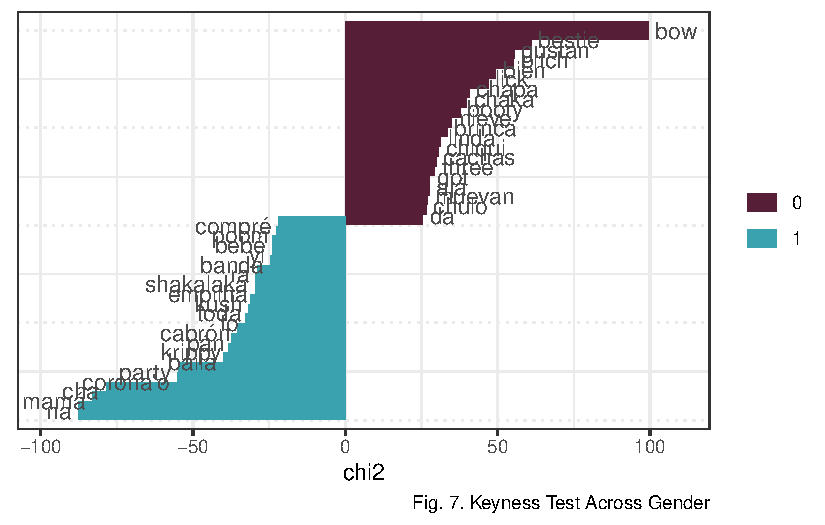
\includegraphics{Sastoque_Essay3_files/figure-pdf/keyness-1.pdf}

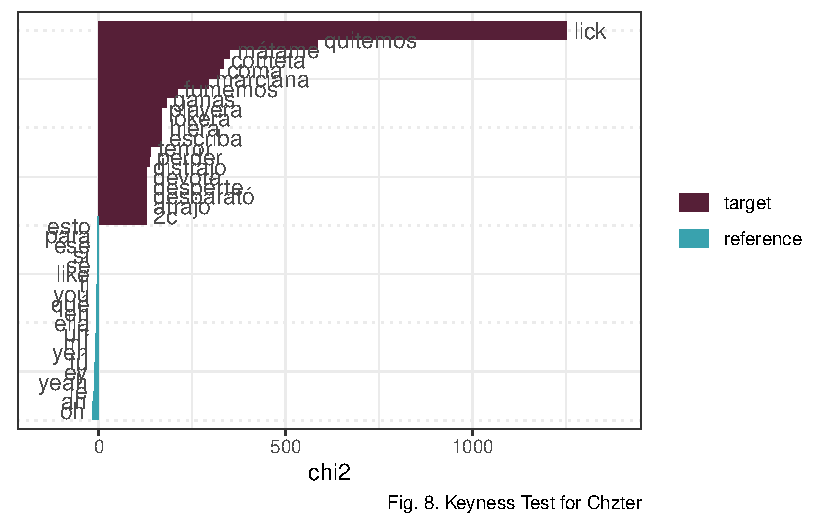
\includegraphics{Sastoque_Essay3_files/figure-pdf/keyness-2.pdf}

\hypertarget{lexical-diversity}{%
\subsubsection{\texorpdfstring{4.4 \textbf{Lexical
Diversity}}{4.4 Lexical Diversity}}\label{lexical-diversity}}

For the purpose of investigating the findings of Torres-Toukoumidis, et
al., this study also computed measures of lexical diversity across the
two groups. This test computes the TTR measure, understood as simply the
ratio of token types to the number of tokens in a given text. For this
corpus, sapphic women's songs presented a higher TTR as compared to men,
which is an interesting addition to the previous findings.

\begin{longtable}[]{@{}ll@{}}
\caption{Table 9. Lexical Diversity Measures Across
Groups}\tabularnewline
\toprule()
Artist\_Gender & mean\_TTR \\
\midrule()
\endfirsthead
\toprule()
Artist\_Gender & mean\_TTR \\
\midrule()
\endhead
Men & 0.3581007 \\
Women & 0.3960211 \\
\bottomrule()
\end{longtable}

\hypertarget{conclusion}{%
\subsection{\texorpdfstring{5
\textbf{Conclusion}}{5 Conclusion}}\label{conclusion}}

\begin{itemize}
\item
  Loop theory back in
\item
  It is hard to make generalizations from the data at hand. The
  repetition of certain phrases especially if a phrase is part of a
  chorus, such as in Young Miko's ``Wiggy'' in \textbf{Table 8,} makes
  it so frequencies can easily become inflated. Token frequencies are
  helpful in hypothesizing ways in which women could be modifying
  conventions of the genre, but it is difficult to assess the actuality
  of these differences. Perhaps a more valuable piece of this analysis
  is the possibility of understanding how certain commonly-used words
  take on different meanings in context, such as ``amiga.'' However,
  since so much of lyrical creativity is a personal choice, it is easier
  to analyze these characteristics through individual case studies, such
  as that of ``Riri'' at the start of this essay. Once more, the domain
  of sapphic urban Latin music resists canonization, and while we may be
  able to develop hypotheses, it is hard to find generalizable traits.
\item
  So much of it is authorial choice.
\item
  Perhaps we can take this an analyses as a motivation to look further
  into how the particular experiences of women affect their use of
  language. With the difficulties in generalization in mind,
  close-reading analyses can approach these texts with less of an
  intention to generalize.
\end{itemize}

\hypertarget{bibliography}{%
\subsection{6 Bibliography}\label{bibliography}}

Acosta-Aguilar, Karina. ``How Reggaeton Is Enabling Self-Expression,
Feminism, and Dismantling Machismo.'' \emph{Medium} (blog), May 4, 2023.
\url{https://medium.com/@karinaacost7/how-reggaeton-is-enabling-self-expression-feminism-and-dismantling-machismo-6462b1a7e588}.

Bode, Katherine. ``The Equivalence of `Close' and `Distant' Reading; or,
Toward a New Object for Data-Rich Literary History.'' \emph{Modern
Language Quarterly (Seattle)} 78, no. 1 (2017): 77--106.
\url{https://doi.org/10.1215/00267929-3699787}.

Byszuk, Joanna. ``The Voices of Doctor Who -- How Stylometry Can Be
Useful in Revealing New Information About TV Series.'' \emph{Digital
Humanities Quarterly} 014, no. 4 (December 20, 2020).

Dediós, Patricio Josué Velarde. ``Reguetón de mujeres para mujeres: dos
caminos de empoderamiento.'' \emph{Antec: Revista Peruana de
Investigación Musical} 5, no. 1 (August 14, 2021): 91--109.
\url{https://doi.org/10.62230/antec.v5i1.112}.

Eder, Maciej, Jan Rybicki, and Mike Kestemont. ``Stylometry with R: A
Package for Computational Text Analysis.'' \emph{The R Journal} 8
(January 1, 2016): 107--21. \url{https://doi.org/10.32614/RJ-2016-007}.

Egbert, Jesse, Douglas Biber, and Bethany Gray. \emph{Designing and
Evaluating Language Corpora: A Practical Framework for Corpus
Representativeness}. Cambridge University Press, 2022.
\url{https://doi.org/10.1017/9781316584880}.

GitHub. ``Distant\_Reading\_in\_R/Text\_Analysis/05a\_Stylometry.R at
Main · ABC-DH/Distant\_Reading\_in\_R.'' Accessed March 8, 2024.
\url{https://github.com/ABC-DH/Distant_Reading_in_R/blob/main/Text_Analysis/05a_Stylometry.R}.

GitHub.
``Hikmah-Academic-Quarto/Examples/Hikmah-Testing-Custom-Manuscript.Pdf
at Main · Andrewheiss/Hikmah-Academic-Quarto.'' Accessed March 8, 2024.
\url{https://github.com/andrewheiss/hikmah-academic-quarto/blob/main/examples/hikmah-testing-custom-manuscript.pdf}.

Goldman, Dara E. ``Walk like a Woman, Talk like a Man: Ivy Queen's
Troubling of Gender.'' \emph{Latino Studies} 15, no. 4 (November 1,
2017): 439--57. \url{https://doi.org/10.1057/s41276-017-0088-5}.

Grosz, Elizabeth. ``Refiguring Lesbian Desire.'' In \emph{Space, Time
and Perversion}. Routledge, 1995.

Hatzel, Hans Ole, Haimo Stiemer, Chris Biemann, and Evelyn Gius.
``Machine Learning in Computational Literary Studies.'' \emph{It -
Information Technology} 65, no. 4--5 (August 1, 2023): 200--217.
\url{https://doi.org/10.1515/itit-2023-0041}.

Houston, Natalie M. ``Distant Reading and Victorian Women's Poetry.'' In
\emph{The Cambridge Companion to Victorian Women's Poetry}, 249--65.
Cambridge University Press, 2019.
\url{https://doi.org/10.1017/9781316856543.017}.

LeBrón, Marisol. ``\,`Con Un Flow Natural': Sonic Affinities and
Reggaeton Nationalism.'' \emph{Women \& Performance: A Journal of
Feminist Theory} 21, no. 2 (July 1, 2011): 219--33.
\url{https://doi.org/10.1080/0740770X.2011.607598}.

Monzingo, Elizabeth, and Daniel Shanahan. ``The Expression of Self and
Grief in the Nineteenth Century: An Analysis through Distant Readings.''
\emph{Nineteenth-Century Music Review} 18, no. 1 (2021): 83--107.
\url{https://doi.org/10.1017/S1479409819000697}.

Mulvey, Laura. ``Visual Pleasure and Narrative Cinema.'' In
\emph{Feminism and Film Theory}, 57--68, 2013.
\url{https://doi.org/10.4324/9780203699362}.

Noriega, Dulce Asela Martínez. ``Música, imagen y sexualidad: el
reggaetón y las asimetrías de género.'' \emph{El Cotidiano}, no. 186
(2014): 63--67.

Rivera-Servera, Ramón H. \emph{Performing Queer Latinidad: Dance,
Sexuality, Politics}. 1st ed.~Triangulations: Lesbian/Gay/Queer
Theater/Drama/Performance. Ann Arbor: University of Michigan Press,
2012. \url{https://doi.org/10.3998/mpub.2395967}.

Showalter, Elaine. ``Feminist Criticism in the Wilderness.''
\emph{Critical Inquiry} 8, no. 2 (1981): 179--205.

Solá-Santiago, Frances. ``Welcome to Young Miko's World.'' \emph{Rolling
Stone} (blog), June 26, 2023.
\url{https://www.rollingstone.com/music/music-features/young-miko-trap-kitty-bad-bunny-karol-g-1234771397/}.

Toro, Ximena de. ``Métele con candela pa' que todas las gatas se muevan.
Identidades de género, cuerpo y sexualidad en el reggaetón.''
\emph{Revista Punto Género}, no. 1 (October 13, 2011).
\url{https://doi.org/10.5354/2735-7473.2011.16824}.

Torres-Toukoumidis, Angel, Cristian Orlando Coronel Quezada, Jenny
Pontón, and Isidro Marín-Gutiérrez. ``Computational Analysis of Latin
Music Songs Through Tokenization. Case of Female Artists and
Reggaeton.'' In \emph{Communication and Applied Technologies}, edited by
Paulo Carlos López-López, Daniel Barredo, Ángel Torres-Toukoumidis,
Andrea De-Santis, and Óscar Avilés, 527--35. Smart Innovation, Systems
and Technologies. Singapore: Springer Nature, 2023.
\url{https://doi.org/10.1007/978-981-19-6347-6_47}.

Vankova, Pavlina. ``Studying the Vocabulary of Reggaeton Song Lyrics.''
\emph{Topics in Linguistics} 23, no. 2 (2022): 63--88.
\url{https://doi.org/10.2478/topling-2022-0012}.



\end{document}
